\hypertarget{the-microwave-innovation-matrix}{%
\section{The microwave innovation matrix}\label{the-microwave-innovation-matrix}}

\begin{figure}[tbp]
\centering
\IfFileExists{figures/0_innovation_matrix.pdf}{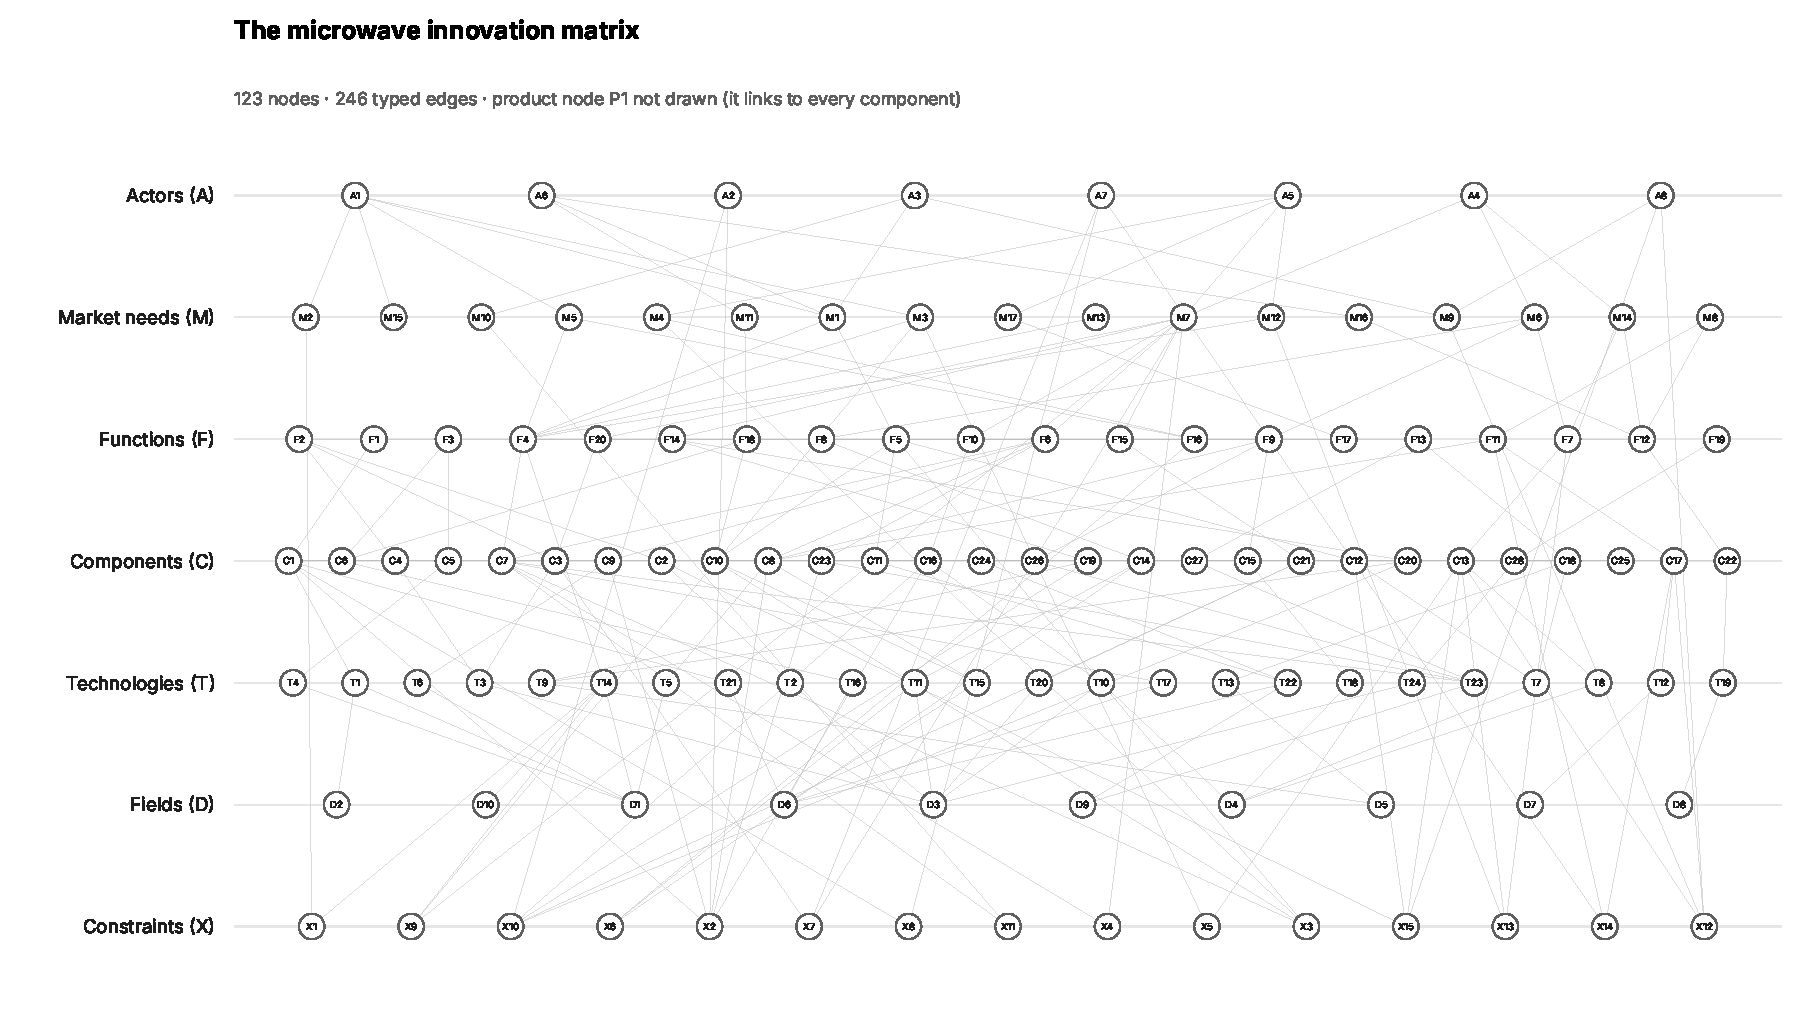
\includegraphics[width=\textwidth]{figures/0_innovation_matrix.pdf}}{\fbox{\parbox[c][5cm][c]{0.9\textwidth}{\centering\small missing: \texttt{\detokenize{figures/0_innovation_matrix.pdf}}}}}
\caption{The full microwave innovation matrix (condition A).}
\label{fig:im_full}
\end{figure}

Figure \ref{fig:im_full} shows the whole graph. All 123 nodes are listed below by layer; the 246 edges and their types are in \texttt{microwave\_base\_graph.yaml}.

\textbf{Market needs (17)}

\begin{longtable}[]{@{}ll@{}}
\toprule\noalign{}
ID & Label \\
\midrule\noalign{}
\endhead
\bottomrule\noalign{}
\endlastfoot
M1 & Fast reheating for busy households \\
M2 & Crispy, browned texture like conventional oven \\
M3 & Hot milk / drink ready for breakfast \\
M4 & Defrost frozen food quickly \\
M5 & Save time in the kitchen \\
M6 & Simple operation with no learning curve \\
M7 & Safe for family use (radiation, burns, electric shock) \\
M8 & Human need for feedback (know when food is ready) \\
M9 & Low purchase price \\
M10 & Small kitchen footprint \\
M11 & Easy to clean \\
M12 & Healthy diet (nutrient retention, less fat) \\
M13 & Energy efficiency \\
M14 & Accessible for elderly / visually impaired users \\
M15 & Appliances that make you feel better (latent need) \\
M16 & Need for mobility (not having to stand by the appliance) \\
M17 & Bake a birthday cake (prep tasks like melting butter) \\
\end{longtable}

\textbf{Functions (20)}

\begin{longtable}[]{@{}
  >{\raggedright\arraybackslash}p{(\columnwidth - 2\tabcolsep) * \real{0.0625}}
  >{\raggedright\arraybackslash}p{(\columnwidth - 2\tabcolsep) * \real{0.9375}}@{}}
\toprule\noalign{}
\begin{minipage}[b]{\linewidth}\raggedright
ID
\end{minipage} & \begin{minipage}[b]{\linewidth}\raggedright
Label
\end{minipage} \\
\midrule\noalign{}
\endhead
\bottomrule\noalign{}
\endlastfoot
F1 & Generates microwave energy at 2.45 GHz \\
F2 & Converts mains voltage to $\sim$4~kV DC for the magnetron \\
F3 & Guides microwave energy into the cavity \\
F4 & Heats food via dielectric water-molecule vibration (FastHeating) \\
F5 & Distributes heat evenly by rotating food through the field \\
F6 & Contains microwave radiation inside the appliance \\
F7 & Sets and counts down cooking duration \\
F8 & Sets average heating power level \\
F9 & Opens and closes the door to access the cavity \\
F10 & Cuts RF power instantly when the door opens \\
F11 & Illuminates cavity so the user can watch the food \\
F12 & Signals end of cooking (audible alert) \\
F13 & Cools magnetron and electronics \\
F14 & Protects against overheating \\
F15 & Protects against overcurrent and electrical faults \\
F16 & Defrosts frozen food (low-power cycling) \\
F17 & Melts / softens butter, chocolate, etc. \\
F18 & Contains spills and allows cleaning \\
F19 & Suppresses electrical noise conducted back to mains \\
F20 & Discharges stored high voltage after switch-off \\
\end{longtable}

\textbf{Components (28)}

\begin{longtable}[]{@{}
  >{\raggedright\arraybackslash}p{(\columnwidth - 2\tabcolsep) * \real{0.0625}}
  >{\raggedright\arraybackslash}p{(\columnwidth - 2\tabcolsep) * \real{0.9375}}@{}}
\toprule\noalign{}
\begin{minipage}[b]{\linewidth}\raggedright
ID
\end{minipage} & \begin{minipage}[b]{\linewidth}\raggedright
Label
\end{minipage} \\
\midrule\noalign{}
\endhead
\bottomrule\noalign{}
\endlastfoot
C1 & Magnetron tube (2.45 GHz, $\sim$700~W output) \\
C2 & High-voltage transformer \\
C3 & High-voltage capacitor ($\sim$1~$\mu$F, 2.1~kV) with internal bleeder resistor \\
C4 & High-voltage rectifier diode \\
C5 & Waveguide duct \\
C6 & Mica waveguide cover \\
C7 & Enamelled steel cooking cavity ($\sim$20~L) \\
C8 & Hinged door with perforated metal mesh window \\
C9 & Door choke seal (quarter-wave rim) \\
C10 & Rotating glass turntable tray \\
C11 & Roller ring and coupler (turntable support) \\
C12 & Turntable motor ($\sim$5~rpm) \\
C13 & Mechanical timer knob \& cam switch (0-30 min) \\
C14 & Power-level knob (5-step duty-cycle cam switch) \\
C15 & Door-release push button \& latch lever \\
C16 & Door interlock microswitches (primary, secondary, monitor) \\
C17 & Interior lamp (20-25 W incandescent) \\
C18 & Cooling fan and fan motor \\
C19 & Magnetron thermal cutout \\
C20 & Cavity thermal cutout \\
C21 & Main ceramic fuse \\
C22 & End-of-cycle bell (mechanical `ding') \\
C23 & Outer steel cabinet (wrapper) \\
C24 & Control panel fascia \\
C25 & Mains power cord and plug \\
C26 & Door hinges \\
C27 & Ventilation louvres \\
C28 & Mains EMI noise filter \\
\end{longtable}

\textbf{Technologies (24)}

\begin{longtable}[]{@{}
  >{\raggedright\arraybackslash}p{(\columnwidth - 2\tabcolsep) * \real{0.0625}}
  >{\raggedright\arraybackslash}p{(\columnwidth - 2\tabcolsep) * \real{0.9375}}@{}}
\toprule\noalign{}
\begin{minipage}[b]{\linewidth}\raggedright
ID
\end{minipage} & \begin{minipage}[b]{\linewidth}\raggedright
Label
\end{minipage} \\
\midrule\noalign{}
\endhead
\bottomrule\noalign{}
\endlastfoot
T1 & Electron cyclotron motion in crossed $E \times B$ fields (cavity magnetron) \\
T2 & Magnetic-shunt leakage HV transformer \\
T3 & Half-wave voltage doubler (capacitor + diode) \\
T4 & Rectangular waveguide TE10 mode propagation \\
T5 & Sub-wavelength aperture shielding (Faraday cage effect) \\
T6 & Quarter-wave choke seal \\
T7 & Shaded-pole / synchronous AC micro-motor (electromagnetic induction) \\
T8 & Motor-driven cam timer with spring-return mechanism \\
T9 & Bimetallic snap-disc thermostat \\
T10 & Redundant interlock microswitch logic (primary / secondary / monitor) \\
T11 & Duty-cycle power modulation (on/off cycling) \\
T12 & Incandescent tungsten-filament lamp \\
T13 & Forced-air convection cooling \\
T14 & Dielectric heating (dipolar rotation of water molecules) \\
T15 & Tempered / borosilicate glass forming \\
T16 & Mica sheet dielectric (muscovite laminate) \\
T17 & Enamel / epoxy powder coating of steel \\
T18 & Spring-loaded lever latch mechanics \\
T19 & Mechanical bell striker \\
T20 & Ceramic cartridge fuse (fusible-link overcurrent protection) \\
T21 & Sintered ferrite permanent magnets \\
T22 & Injection-molded engineering thermoplastics (PP, PBT, PPS) \\
T23 & Sheet-steel stamping \& spot welding \\
T24 & Passive LC EMI line filtering \\
\end{longtable}

\textbf{Fields (10)}

\begin{longtable}[]{@{}ll@{}}
\toprule\noalign{}
ID & Label \\
\midrule\noalign{}
\endhead
\bottomrule\noalign{}
\endlastfoot
D1 & Radio-frequency \& microwave engineering \\
D2 & Vacuum electronics \\
D3 & Power electronics \& electrical engineering \\
D4 & Electromechanics \& mechanisms \\
D5 & Thermal engineering \& heat transfer \\
D6 & Materials science (metals, ceramics, glass, polymers) \\
D7 & Lighting \& optics \\
D8 & Sound engineering \\
D9 & Manufacturing engineering (stamping, molding, assembly) \\
D10 & Food science (dielectric properties of food) \\
\end{longtable}

\textbf{Constraints (15)}

\begin{longtable}[]{@{}
  >{\raggedright\arraybackslash}p{(\columnwidth - 2\tabcolsep) * \real{0.0625}}
  >{\raggedright\arraybackslash}p{(\columnwidth - 2\tabcolsep) * \real{0.9375}}@{}}
\toprule\noalign{}
\begin{minipage}[b]{\linewidth}\raggedright
ID
\end{minipage} & \begin{minipage}[b]{\linewidth}\raggedright
Label
\end{minipage} \\
\midrule\noalign{}
\endhead
\bottomrule\noalign{}
\endlastfoot
X1 & Microwaves can't brown or crisp food surfaces \\
X2 & FCC/FDA radiation-leakage safety limits (21 CFR 1030.10, 5~mW/cm\textsuperscript{2} at 5~cm) \\
X3 & Uneven heating --- standing-wave hot and cold spots \\
X4 & Metal objects in cavity cause arcing \\
X5 & Mechanical timer imprecise for short (\textless1 min) durations \\
X6 & Power only adjustable by on/off cycling, not continuously \\
X7 & HV capacitor can hold a lethal charge after unplugging \\
X8 & Limited magnetron lifetime (cathode/filament wear) \\
X9 & Superheating of liquids --- risk of eruptive boiling \\
X10 & Electrical safety standards (IEC 60335-2-25 / UL 923) \\
X11 & Cavity volume limited by countertop size \\
X12 & Low BOM target for entry-level price segment \\
X13 & No food-state sensing --- open-loop cooking \\
X14 & Interior lamp burns out and is hard to replace \\
X15 & Regional mains variants (230 V/50 Hz vs 120 V/60 Hz) \\
\end{longtable}

\textbf{Actors (8)}

\begin{longtable}[]{@{}ll@{}}
\toprule\noalign{}
ID & Label \\
\midrule\noalign{}
\endhead
\bottomrule\noalign{}
\endlastfoot
A1 & Time-pressed home cook \\
A2 & Appliance safety regulator/inspector \\
A3 & Student / single-person household \\
A4 & Elderly user \\
A5 & Parent with young children \\
A6 & Office worker using a shared kitchen \\
A7 & Repair technician \\
A8 & OEM manufacturer / cost engineer \\
\end{longtable}

\textbf{Product (1)}

\begin{longtable}[]{@{}
  >{\raggedright\arraybackslash}p{(\columnwidth - 2\tabcolsep) * \real{0.0625}}
  >{\raggedright\arraybackslash}p{(\columnwidth - 2\tabcolsep) * \real{0.9375}}@{}}
\toprule\noalign{}
\begin{minipage}[b]{\linewidth}\raggedright
ID
\end{minipage} & \begin{minipage}[b]{\linewidth}\raggedright
Label
\end{minipage} \\
\midrule\noalign{}
\endhead
\bottomrule\noalign{}
\endlastfoot
P1 & Basic countertop microwave oven (timer knob, power knob, door button, lamp) \\
\end{longtable}

\hypertarget{generation-prompt}{%
\section{Generation prompt}\label{generation-prompt}}

The template used for every call (\texttt{template\_prompt.txt}). Placeholders in braces are filled per call; the opening sentence of the system prompt is shown filled in.

\begin{verbatim}
=== SYSTEM ===
You are an innovation engineer. You read product graphs and propose radical
product innovations. Respond with valid JSON only, no prose outside the JSON.

=== USER ===
Innovate the following {product_name} based on the graph given.
Encourage radical and wild ideas.

TARGET MARKET NEED
{target_need_id}: {target_need_label}
Favour innovations that serve this market need.

INNOVATION OPERATOR: {operator_name}
{operator_definition}

EXAMPLE OF AN INNOVATION WE LIKE
A microwave has a door with holes, a light, and other components and
functions, so the user can see inside: they need to check for mistakes
(perhaps there is also entertainment value).
Applying the operator: replace the light and the holes with something
that fulfils the same function equally well or better, or more cheaply.
  - e.g. 1: a webcam
  - e.g. 2: a fully transparent microwave casing that needs no light bulb inside

GRAPH OF THE {product_name}
{graph_yaml}

OUTPUT
Return exactly {n_ideas} ideas as JSON:
{
  "ideas": [
    {
      "title": "short name",
      "anchors": ["existing node ids the operator was applied to"],
      "new_nodes": [
        {"type": "Field|Technology|Component|Function|MarketNeed|Constraint",
         "label": "...", "detail": "one line"}
      ],
      "new_edges": [
        {"from": "node id or new node label", "to": "node id or new node label",
         "type": "one of the graph's edge_types, e.g. resolves"}
      ],
      "rationale": "one sentence: how this serves {target_need_id}"
    }
  ]
}
\end{verbatim}

\hypertarget{pairwise-judge-prompt}{%
\section{Pairwise judge prompt}\label{pairwise-judge-prompt}}

System prompt:

\begin{verbatim}
You are an expert panel judging product-innovation brainstorming. You compare two sets of ideas produced for the same brief. Judge only the ideas themselves; ignore length and formatting. Respond with valid JSON only.
\end{verbatim}

User prompt:

\begin{verbatim}
BRIEF
Product: {product}
Target market need: {need_id}: {need_label}
Innovation operator: {operator}
The brief asked for radical, wild ideas that serve the target need.

SET 1
{set1}

SET 2
{set2}

Score each set from 1 (poor) to 5 (excellent) on:
- relevance: how well the ideas serve the target need
- novelty: how radical and non-obvious the ideas are
- feasibility: how technically plausible the ideas are
- specificity: how concrete the ideas are (named components, mechanisms)
- diversity: how different the ideas are from each other

Then pick the better set overall for this brief.

Return JSON:
{"set_1": {"relevance": 0, "novelty": 0, "feasibility": 0, "specificity": 0, "diversity": 0},
 "set_2": {"relevance": 0, "novelty": 0, "feasibility": 0, "specificity": 0, "diversity": 0},
 "winner": "set_1" | "set_2" | "tie",
 "reason": "one sentence"}
\end{verbatim}

\hypertarget{individual-scoring-prompts}{%
\section{Individual scoring prompts}\label{individual-scoring-prompts}}

Quality, used for every idea. System prompt:

\begin{verbatim}
You are an expert panel judging product-innovation ideas. Rate each idea on its own merits, independently of the others. Ignore writing style and length. Respond with valid JSON only.
\end{verbatim}

User prompt:

\begin{verbatim}
BRIEF
Product: {product}
Target market need: {need_id}: {need_label}
Innovation operator: {operator}
The brief asked for radical, wild ideas that serve the target need.

IDEAS
{ideas}

Rate EACH idea from 1 (poor) to 5 (excellent) on:
- relevance: how well it serves the target need
- novelty: how radical and non-obvious it is
- feasibility: how technically plausible it is
- specificity: how concrete it is (named components, mechanisms)

Return JSON with one entry per idea, in the same order:
{"ratings": [{"idea": 1, "relevance": 0, "novelty": 0, "feasibility": 0, "specificity": 0,
               "comment": "one sentence"}]}
\end{verbatim}

\hypertarget{data-and-code}{%
\section{Data and code}\label{data-and-code}}

The project repository (\url{https://github.com/orioli/IM-LLM}) is organized as follows:

\begin{longtable}[]{@{}
  >{\raggedright\arraybackslash}p{(\columnwidth - 2\tabcolsep) * \real{0.3800}}
  >{\raggedright\arraybackslash}p{(\columnwidth - 2\tabcolsep) * \real{0.6200}}@{}}
\toprule\noalign{}
\begin{minipage}[b]{\linewidth}\raggedright
Component / Path
\end{minipage} & \begin{minipage}[b]{\linewidth}\raggedright
Contents \& Role
\end{minipage} \\
\midrule\noalign{}
\endhead
\bottomrule\noalign{}
\endlastfoot
\texttt{microwave\_base\_graph.yaml} & Full innovation matrix (123 nodes, 246 typed edges) \\
\texttt{slicer.py}, \texttt{slices/} & Graph slicer generating vertical slices (B) and random slices (R) with \texttt{manifest.csv} \\
\texttt{KG\_informed\_brainstorm\_AB\_Test.py} & Ideation execution harness across conditions and effort levels \\
\texttt{analyze.py}, \texttt{top\_ideas.py} & Pairwise set judging and individual quality scoring harnesses \\
\texttt{runs/rq1\_full.jsonl} & Complete raw call logs (580 runs, 2,892 ideas, prompt hashes, token counts) \\
\texttt{results/judgments.jsonl}, \texttt{results/idea\_scores.jsonl} & Raw blind judge evaluations and point scores \\
\texttt{results/pairwise\_summary.csv}, \texttt{results/tail\_summary.csv} & Summary statistics, win rates, and bootstrap yield slope estimates \\
\texttt{yield\_per\_market\_need.xlsx} & Per-market-need top ideas, tokens, yields, and sign tests (live spreadsheet formulas) \\
\texttt{render\_matrix\_v2.py}, \texttt{*.html} & Interactive visualizers for exploring the full matrix and subgraph slices \\
\texttt{charts.py}, \texttt{tail\_charts.py} & Figure and visualization generation scripts \\
\texttt{build\_paper.py} & Automated end-to-end manuscript build, data verification, and compilation pipeline \\
\end{longtable}
